\documentclass[t]{beamer}
\usetheme{Copenhagen}
\setbeamertemplate{headline}{} % remove toc from headers
\beamertemplatenavigationsymbolsempty

\usepackage{amsmath, array, tikz, bm, pgfplots, tcolorbox, graphicx}
\pgfplotsset{compat = 1.16}

\title{Measures of Position}
\author{}
\date{}

\AtBeginSection[]
{
  \begin{frame}
    \frametitle{Objectives}
    \tableofcontents[currentsection]
  \end{frame}
}

\begin{document}

\begin{frame} 
\maketitle
\end{frame}

\section{Use z-scores to compare data values}

\begin{frame}{z-scores}
\begin{tcolorbox}[colframe=green!20!black, colback = green!30!white,title=\textbf{z-score}]
A \textbf{z-score} (a.k.a. \textbf{standard score}) measures how many standard deviations a data value, $x$, is from the mean of the data set.
\end{tcolorbox}
\vspace{8pt}	\pause
\begin{itemize}
	\item A positive z-score indicates an above average value.	\newline\\	\pause
	\item A negative z-score indicates a below average value.	\newline\\	\pause
	\item A z-score of 0 indicates an exact average value.
\end{itemize}
\end{frame}

\begin{frame}{Visual Interpretation of z-Scores}
\begin{center}
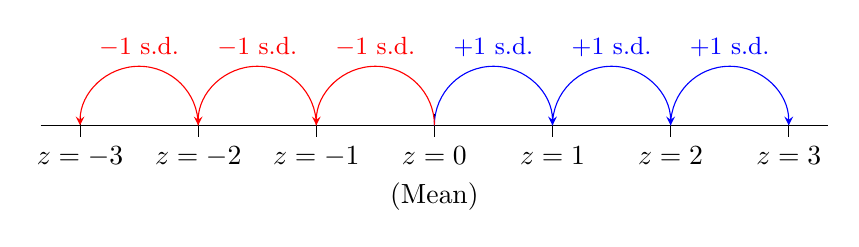
\begin{tikzpicture}
\draw (-5,0) -- (5,0);
\foreach \x in {-4.5,-3,...,4.5}
\draw (\x, 0.15) -- (\x, -0.15);
\node at (0,-0.15) [below] {$z=0$};
\node at (0,-0.6) [below] {(Mean)};
\node at (1.5,-0.15) [below] {$z=1$};
\draw [->, >=stealth,blue] (0,0) arc (180:0:0.75) node [above, midway] {\small$+1\text{ s.d.}$};
\node at (3,-0.15) [below] {$z=2$};
\draw [->, >=stealth,blue] (1.5,0) arc (180:0:0.75) node [above, midway] {\small$+1\text{ s.d.}$};
\node at (4.5,-0.15) [below] {$z=3$};
\draw [->, >=stealth,blue] (3,0) arc (180:0:0.75) node [above, midway] {\small$+1\text{ s.d.}$};
\node at (-1.5,-0.15) [below] {$z=-1$};
\draw [->, >=stealth, red] (0,0) arc (0:180:0.75) node [above, midway] {\small$-1\text{ s.d.}$};
\node at (-3,-0.15) [below] {$z=-2$};
\draw [->, >=stealth, red] (-1.5,0) arc (0:180:0.75) node [above, midway] {\small$-1\text{ s.d.}$};
\node at (-4.5,-0.15) [below] {$z=-3$};
\draw [->, >=stealth, red] (-3,0) arc (0:180:0.75) node [above, midway] {\small$-1\text{ s.d.}$};
\end{tikzpicture}
\end{center}
\end{frame}

\begin{frame}{z-Score Formula}
\[z = \frac{x-\mu}{\sigma}\]	\pause

z-scores can compare two different data sets that use different scales of measurement.	\newline\\	\pause

``Usual" data values have z-scores between $-2$ and 2.
\end{frame}

\begin{frame}{Example 1}
The mean SAT score is 1059 with a standard deviation of 210; meanwhile the mean ACT score is 21 with a standard deviation of 5.4. A student takes both tests and receives a 1350 on the SAT and a 29 on the ACT. On which test did the student score better? \\
\begin{align*}
\onslide<2->{z_{\text{SAT}} &= \frac{1350-1059}{210}}	&	\onslide<4->{z_{\text{ACT}} &= \frac{29-21}{5.4}}	\\[10pt]
\onslide<3->{z_{\text{SAT}} &= 1.39}					&	\onslide<5->{z_{\text{ACT}} &= 1.48}	\\
\end{align*}
\onslide<6->{The student did relatively better on the ACT.}
\end{frame}


\section{Determine and interpret percentiles}

\begin{frame}{Percentiles}
\begin{tcolorbox}[colframe=green!20!black, colback = green!30!white,title=\textbf{Percentile}]
A \textbf{percentile} is a measure of location that divide a set of data into 100 groups with about 1\% of the values in each group.
\end{tcolorbox}
\vspace{11pt} \pause

\begin{tcolorbox}[colframe=green!20!black, colback = green!30!white,title=\textbf{Percentile Score}]
A \textbf{percentile score} is the percent of data values less than a given value. (\emph{Note}: this is \underline{not} the same as percentage).
\end{tcolorbox}
\end{frame}

\begin{frame}{Example 2}
For the dataset below, determine the percentile score for the data value 28.
\begin{center}
30, 35, 28, 28, 19, 21, 34, 7, 21, 9, 36, 29, 33, 35, 13
\end{center}
\vspace{8pt}	\pause
First, sort the dataset:
\begin{center}
7, 9, 13, 19, 21, 21, 28, 28, 29, 30, 33, 34, 35, 35, 36
\end{center}
\vspace{8pt}	\pause
There are 6 data values less than 28 in the dataset with 15 values: \quad $6/15 = 40\%$	\newline\\	\pause
28 is in the 40th percentile.
\end{frame}

\begin{frame}{Methods}
\textbf{Bad News:}	\newline\\
There isn't a universally agreed upon method for finding percentiles.	\newline\\	\pause
\textbf{Good News:}	\newline\\	
Differences in percentile calculations become negligible for larger datasets.
\end{frame}

\begin{frame}{Visualization of Percentiles}
Eventually, we will think of being in the 40th percentile as something like the following:	
\begin{center}
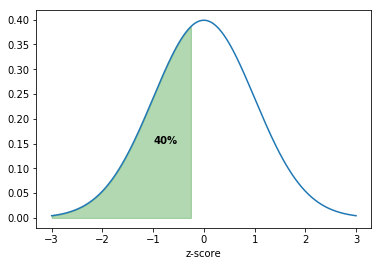
\includegraphics[scale=0.6]{../Images/percentile.png}
\end{center}
\end{frame}

\begin{frame}{Example 3}
What is the difference between scoring 90\% on a test and being in the 90th percentile for that test?	\newline\\	\pause

Scoring 90\% on the test means you earned 90\% of the total available points on the test.	\newline\\	\pause

Scoring in the 90th percentile means you did better on the test than 90\% of everyone else who took it.
\end{frame}

\section{Determine the five-number summary}

\section{Create a boxpolot of a dataset}
\end{document}